\documentclass[12pt]{article}
\usepackage[utf8]{inputenc}
\usepackage[a4paper,margin=1in]{geometry}
\usepackage{amsmath,amssymb}
\usepackage{enumitem,parskip,hyperref,xcolor,fancyhdr,tikz,graphicx,eso-pic,titlesec}
\graphicspath{{../}}
\definecolor{kcpc-text}{RGB}{20,20,20}
\definecolor{kcpc-muted}{RGB}{90,90,90}
\definecolor{kcpc-red}{RGB}{176,0,0}
\pagestyle{fancy}\fancyhf{}
\lhead{\textcolor{kcpc-text}{\small\bfseries Problems}}
\rhead{\textcolor{kcpc-muted}{\small Week 5}}
\cfoot{\textcolor{kcpc-muted}{\small KCPC}}
\renewcommand{\headrulewidth}{0.4pt}
\renewcommand{\headrule}{\hbox to\headwidth{\color{kcpc-red}\leaders\hrule height \headrulewidth\hfill}}
\renewcommand{\footrulewidth}{0pt}
\setlength{\headheight}{28pt}
\AddToShipoutPictureBG{\begin{tikzpicture}[remember picture,overlay]
  \node[opacity=0.035,at=(current page.center)]{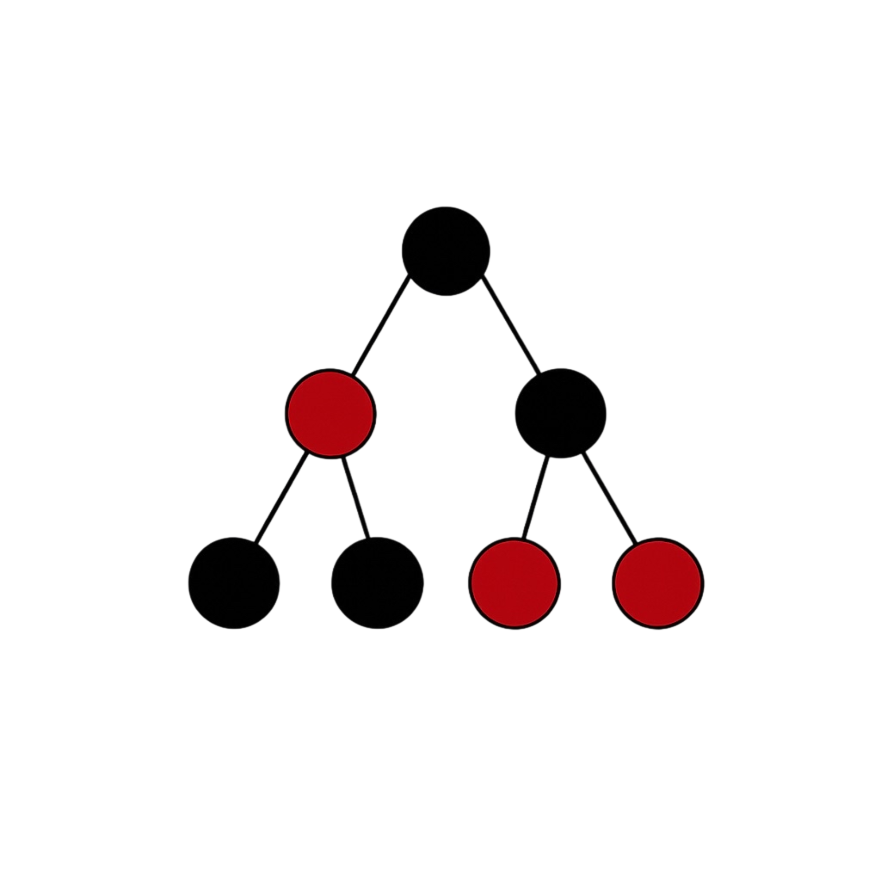
\includegraphics[width=0.38\paperwidth]{kcpc-logo.png}};
\end{tikzpicture}}
\titleformat{\section}{\large\bfseries\color{kcpc-red}}{\thesection}{1em}{}
\setlist[itemize]{noitemsep,topsep=4pt}
\setlist[enumerate]{topsep=4pt}
\hypersetup{colorlinks=true,urlcolor=kcpc-red,linkcolor=kcpc-red}
\title{KCPC Week 5 Problems\\Graphs II: Dijkstra and 0--1 BFS}
\author{}\date{}

\begin{document}
\maketitle\thispagestyle{fancy}

This sheet accompanies the \emph{Graphs II} workshop, hosted in collaboration with KCL Tech. Problems are divided into three categories, numbered continuously~1--15 to match the slides and the solutions document:
\begin{itemize}
  \item \textbf{Integrated examples (1--3)}: discussed live during the workshop.
  \item \textbf{Core practice (4--11)}: attempted during the workshop, then finished independently.
  \item \textbf{Extended homework (12--15)}: stretch challenges for after the session.
\end{itemize}

\textbf{How to approach every problem.} Before coding, write down the four modelling decisions from the slides:
\begin{enumerate}
  \item \textbf{State}: what is a vertex (a city, a grid cell, a city--time pair, \ldots)?
  \item \textbf{Legal moves}: what are the edges, and are they directed?
  \item \textbf{Move cost}: uniform, binary $\{0,1\}$, or general non-negative?
  \item \textbf{Initial score}: single source or many; is the starting cell itself charged?
\end{enumerate}
Then choose the algorithm by the model, not by the problem's title: uniform positive cost $\Rightarrow$ BFS; costs in $\{0,1\}$ $\Rightarrow$ 0--1 BFS; general non-negative costs $\Rightarrow$ Dijkstra. For maximisation or bottleneck objectives, adapt the relaxation and the heap ordering, and justify why a current best pop is final.

\section*{I. Integrated examples (live walkthroughs)}

\subsection*{1. \href{https://www.geeksforgeeks.org/problems/implementing-dijkstra-set-1-adjacency-matrix/1}{GeeksForGeeks --- Implementing Dijkstra}}
\textbf{Modelling cue:} undirected non-negative weights; return every distance from the source.

\textbf{Note.} The historical title says \emph{Adjacency Matrix}, but the current judge interface is an \textbf{edge list}: \texttt{dijkstra(V, edges, src)} with rows \texttt{[u, v, w]}. Build both adjacency directions.

\subsection*{2. \href{https://leetcode.com/problems/network-delay-time/}{LeetCode 743 --- Network Delay Time}}
\textbf{Modelling cue:} directed edges; a vertex's receive time is its shortest distance; answer is the maximum distance, or $-1$ if any vertex is unreachable. Labels are 1-based.

\subsection*{3. \href{https://leetcode.com/problems/minimum-cost-to-make-at-least-one-valid-path-in-a-grid/}{LeetCode 1368 --- Minimum Cost to Make at Least One Valid Path in a Grid}}
\textbf{Modelling cue:} leaving a cell costs 0 along its arrow and 1 otherwise; the arrow belongs to the cell you \emph{leave}. Use 0--1 BFS.

\section*{II. Core practice}

\subsection*{4. \href{https://leetcode.com/problems/path-with-maximum-probability/}{LeetCode 1514 --- Path with Maximum Probability}}
\textbf{Modelling cue:} maximise a \emph{product} of probabilities, not a sum. Extend by multiplying; use a max-heap (negate keys in Python).

\subsection*{5. \href{https://leetcode.com/problems/path-with-minimum-effort/}{LeetCode 1631 --- Path with Minimum Effort}}
\textbf{Modelling cue:} minimise the \emph{largest} height difference on the path. Extend with $\max(\mathrm{effort}[u], |h[u]-h[v]|)$; keep a min-heap.

\subsection*{6. \href{https://leetcode.com/problems/minimum-obstacle-removal-to-reach-corner/}{LeetCode 2290 --- Minimum Obstacle Removal to Reach Corner}}
\textbf{Modelling cue:} the cost belongs to the \emph{destination} cell: entering an obstacle costs 1. Use 0--1 BFS. Both endpoints are empty.

\subsection*{7. \href{https://leetcode.com/problems/01-matrix/}{LeetCode 542 --- 01 Matrix}}
\textbf{Modelling cue:} multi-source \emph{ordinary} BFS: enqueue every zero at distance 0; first discovery in FIFO order is minimal. Not a 0--1 BFS problem.

\subsection*{8. \href{https://atcoder.jp/contests/abc176/tasks/abc176_d}{AtCoder ABC176 D --- Wizard in Maze}}
\textbf{Modelling cue:} walking to an open orthogonal neighbour costs 0; warping to any open cell with $|\Delta r|\le2$ and $|\Delta c|\le2$ (including corners) costs 1. Use 0--1 BFS. Input coordinates are 1-based; output $-1$ if unreachable.

\subsection*{9. \href{https://projecteuler.net/problem=81}{Project Euler 81 --- Path Sum: Two Ways}}
\textbf{Modelling cue:} moves are right and down only; entering a cell costs its value, including the starting cell. A row-by-row DP also works on this DAG.

\subsection*{10. \href{https://projecteuler.net/problem=82}{Project Euler 82 --- Path Sum: Three Ways}}
\textbf{Modelling cue:} moves are up, down and right; \emph{any} left-column cell may start (seed each at its own value) and \emph{any} right-column cell may finish.

\subsection*{11. \href{https://projecteuler.net/problem=83}{Project Euler 83 --- Path Sum: Four Ways}}
\textbf{Modelling cue:} all four orthogonal moves; top left to bottom right; destination-entry costs. Use Dijkstra (or 0--1 reasoning does \emph{not} apply: values are general positives).

\section*{III. Extended homework}

\textbf{Important.} The following problems are genuinely extremely difficult. Attempt them only after completing all previously listed problems and the assigned supplementary reading. They are stretch challenges for exploring advanced modelling and optimisation techniques. Solutions are provided in C++.

\subsection*{12. \href{https://leetcode.com/problems/minimum-cost-to-reach-destination-in-time/}{LeetCode 1928 --- Minimum Cost to Reach Destination in Time}}
\textbf{Modelling cue:} state expansion: the cheapest arrival at a city may be too slow to finish. Keep $(\mathrm{city}, \mathrm{timeUsed})$ in the state; the source fee and each entered city's fee are charged.

\subsection*{13. \href{https://codeforces.com/problemset/problem/786/B}{Codeforces 786B --- Legacy}}
\textbf{Modelling cue:} segment-tree graph construction with \emph{two directed trees} (out-tree and in-tree sharing original leaves) plus Dijkstra. Do not expand ranges into individual edges.

\subsection*{14. \href{https://codeforces.com/problemset/problem/715/B}{Codeforces 715B --- Complete The Graph}}
\textbf{Modelling cue:} constructive weights: activate missing edges one at a time (weight 1 vs.\ disabled at $L+1$), binary-search the pivot whose activation crosses the target distance, then adjust only the pivot. Vertices are 0-based; input weight 0 means \emph{unknown}.

\subsection*{15. \href{https://atcoder.jp/contests/abc213/tasks/abc213_e}{AtCoder ABC213 E --- Stronger Takahashi}}
\textbf{Modelling cue:} advanced 0--1 movement modelling: one punch clears a $2\times2$ square. Free edges enter only originally open orthogonal neighbours; paid edges use every nonzero offset in the $5\times5$ square \emph{except} the four corners $(\pm2,\pm2)$, and may land on walls.

\end{document}
